% !TeX encoding = windows-1251
\documentclass[a4paper,12pt]{article}
\usepackage{newlistok}
\usepackage{tikz}
\usetikzlibrary{calc}

\global\addtolength{\vsize}{-115mm}%
\global\advance\vsize by 10cm
\global\advance\vsize by 10cm

\ВключитьКолонитул

%\УвеличитьВысоту{1.5cm}
%\УвеличитьШирину{1.5cm}
%\renewcommand{\spacer}{\vfil}

\Заголовок{Неравенства и оценки}
\НомерЛистка{12}
\ДатаЛистка{04.2013}

\begin{document}
\СоздатьЗаголовок


\задача
Что больше:
\пункт
$5^{15}$ или $15^5$;
\пункт
$2^{100}$ или $10^{30}$;
\пункт
$7^8$ или $8^7$;
\пункт
$3^{500}$ или $7^{300}$?
\кзадача

\задача
\пункт
Докажите, что $a+\dfrac1a\geqslant2$ при всех $a>0$.\\
\пункт
Каково наименьшее значение выражения $a+\dfrac9a$ при $a>0$?
\кзадача

\задача
Десятичная запись натурального числа~$a$ состоит из $n$~цифр, а~десятичная запись числа~$a^3$ состоит из $m$~цифр.
\невСтрочку
\пункт
Какие значения может принимать~$m$, если $n$~фиксировано?
\пункт
Может ли $n+m$ быть равным $2013$?
\кзадача

\задача
Число~$x$ изменили не более, чем на~$0.1$. Могло ли при этом измениться более, чем на $10$, значение
\пункт
$x^2$;
\пункт
$\sqrt x$?
\кзадача

\задача
Вкладчик кладёт в~банк $1000$~рублей. В~каком случае спустя 10~лет он получит больше денег: если банк начисляет~$5\%$ от имеющейся суммы один раз в~год или если банк начисляет~$(5/12)\%$ один раз в~месяц?
\кзадача

\задача
Описанный около круга квадрат разбили на $1000\times1000$ равных квадратиков и~закрасили квадратики, не выходящие за пределы круга. Докажите, что площадь получившейся закрашенной фигуры составляет не менее $90\%$ от площади всего круга.
\кзадача

\задача
Докажите, что если $n\in\N$ и~$a>0$, то\\
\пункт
$(1+a)^n\geqslant 1+na$;
\пункт
$(1+a)^n\geqslant 1+na+\frac12n(n-1)a^2$.\\
Какова связь этой задачи с~неравенством Бернулли и~биномом Ньютона?
\кзадача

\задача
Укажите такое натуральное $n>1$, что\\
\пункт
$(1.001)^n>1000$;
\пункт
$(0.999)^n<10^{-10}$;
\пункт
$\sqrt{n+1} - \sqrt n < 0.1$;
\спункт
$\sqrt[n]{n} < 1.001$.
\кзадача

\опр
Говорят, что неравенство выполнено \emph{при всех достаточно
больших~$n$} или \emph{при~$n$ много большем нуля}, если найдётся
такое число~$k$, что данное неравенство выполнено при всех $n>k$.
Обозначение: $n\gg 0$.
\копр

\задача
Докажите, что если $a>1$ и $C\in\R$, то при $n\gg0$
\пункт
$a^n>C$;
\пункт
$a^n>Cn$.
\кзадача

\задача
Докажите, что
\пункт
$2^n>n^{100}$ при $n\gg0$;\\
\пункт
если $a>1$ и~$k$\т натуральное число, то $a^n>n^k$ при $n\gg0$.
\кзадача

\задача
Докажите, что для любого $a\in\R$ неравенство $n!>a^n$ выполнено при $n\gg 0$.
\кзадача

\задача
\пункт
Докажите, что неравенство $n^n>1000n!$ выполнено при $n\gg 0$.\\
\пункт
Останется ли верным это неравенство, если 1000 заменить на произвольное число $C\in\R$?
\кзадача

\задача
Пусть $P(x)=p_n x^n+\ldots+p_0$ и~$Q(x)=q_m x^m+\ldots+q_0$\т многочлены степеней~$n$ и~$m$ соответственно, причём $n>m$ и $p_n,q_m>0$. Докажите, что $P(x)>Q(x)$ при $x\gg 0$.
\кзадача

\vfill
\ЛичныйКондуит{0mm}{6mm}
\ОбнулитьКондуит
\newpage

\задача
Докажите, что при любом натуральном~$n$ справедливо неравенство:\\
\пункт
$\dfrac1{n+1}+\dfrac1{n+2}+\ldots+\dfrac1{2n}\geqslant\dfrac12$;
\пункт
$\dfrac1{1\cdot2}+\dfrac1{2\cdot3}+\ldots+\dfrac1{n\cdot(n+1)}<1$.
\кзадача

\задача
Верно ли, что для любого числа~$C$ найдётся такое натуральное число~$n$, что выполнено неравенство:
\пункт[Гармонический ряд]
$1+\dfrac12+\ldots+\dfrac1n\geqslant C$;
\пункт
$1+\dfrac1{2^2}+\ldots+\dfrac1{n^2}\geqslant C$?
\кзадача

\putthere{165mm}{-10mm}{%
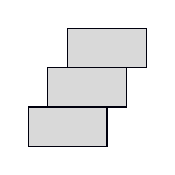
\begin{tikzpicture}[
        x=0.5cm,y=0.5cm
        ,face/.style={draw=blue!5!black,fill=gray!30,thin}
    ]
    \coordinate (ex) at (2,0);
    \coordinate (ey) at (0,1);
    \coordinate (mey) at ($ -1*(ey) $);
    \coordinate (dx) at (0.5,0);
    % Левый нижний угол кирпича
    \coordinate (A) at (0,0);
    \coordinate (B) at ($ (A) + (dx) + (ey) $);
    \coordinate (C) at ($ (B) + (dx) + (ey) $);
    % Кирпичи
    \filldraw[face] (A) -- ++(ey) -- ++(ex) -- ++(mey) -- cycle;
    \filldraw[face] (B) -- ++(ey) -- ++(ex) -- ++(mey) -- cycle;
    \filldraw[face] (C) -- ++(ey) -- ++(ex) -- ++(mey) -- cycle;
\end{tikzpicture}
}{75mm}{}
\vspace{-6mm}

\УстановитьГраницы{0cm}{3.2cm}
\сзадача
Есть неограниченное число одинаковых кирпичей в форме прямоугольного параллелепипеда. Кирпичи кладут друг на друга со сдвигом так, чтобы они
не падали (см.~рис.). \лк Крышу\пк\ какой наибольшей длины можно так получить?\\
\кзадача
\ВосстановитьГраницы

\vspace{-6mm}

\задача
Пусть $a,b>0$ и~$n\in\N$. Докажите неравенство $\dfrac{a^{n+1}}{b^n}\geqslant(n+1)a-nb$.
\кзадача

\задача
Для всех натуральных $n$ докажите следующие неравенства:\\
\пункт
$(1+\frac{1}{n+1})^{n+1}\geqslant(1+\frac{1}{n})^n$;
\пункт
$(1+\frac{1}{n})^{n+1}\leqslant(1+\frac{1}{n-1})^n$;
\пункт
$2\leqslant(1+\frac{1}{n})^n\leqslant4$;
\спункт
$(1+\frac1n)^n\leqslant 3$.
\кзадача

\сзадача
Докажите, что для любого натурального числа~$n$ выполнены неравенства
$$
\left(\dfrac n4\right)^n\leqslant n!\leqslant\left(\dfrac{n+1}2\right)^n.
$$
\кзадача
\vspace{-6mm}

\сзадача[Неравенство Коши]
Докажите, что если $n\in\N$ и~$a_1,a_2,\ldots,a_n>0$, то
$$
\frac{a_1+a_2+\ldots+a_n}{n}\geqslant\sqrt[n]{a_1a_2\ldots a_n}.
$$
\кзадача
\vspace{-6mm}

\задача
Пусть $P(x) = x^{n_1} - x^{n_2} + x^{n_3} - x^{n_4} + \cdots + x^{n_{2k + 1}}$, где $n_1 > n_2 > \cdots > n_{2k + 1}$\т набор натуральных чисел. Докажите что $P(x) \geq 0$ при всех $x > 0$.
\кзадача

\сзадача
Найдите наименьшее значение выражения $\sqrt{(x-1)^2+y^2}+\sqrt{x^2+(y-1)^2}$. При каких $x$ и~$y$ оно достигается?
\кзадача

\сзадача
Коэффициенты $p$ и $q$ квадратного уравнения $x^2+px+q=0$ изменили не больше, чем на 0.01. Мог ли больший корень уравнения измениться больше, чем на 100? \кзадача

\сзадача
Найдётся ли такое натуральное~$n$, что первыми девятью знаками после запятой в~десятичной записи числа $\{\sqrt{n}\}$ будут цифры $987654321$?
\кзадача

\vfill
\ЛичныйКондуит{0mm}{6mm}

%\GenXMLW

\end{document}




